\documentclass[tikz,border=6pt]{standalone}
\usetikzlibrary{arrows.meta,positioning,calc,backgrounds}

\definecolor{envpink}{RGB}{236,204,204}
\definecolor{infgreen}{RGB}{205,223,198}
\definecolor{actblue}{RGB}{190,208,236}
\definecolor{obsgreen}{RGB}{208,226,191}
\definecolor{thinkviolet}{RGB}{215,201,224}
\definecolor{solred}{RGB}{238,196,196}
\definecolor{judgepink}{RGB}{241,210,204}
\definecolor{trainerblue}{RGB}{198,212,235}

\begin{document}
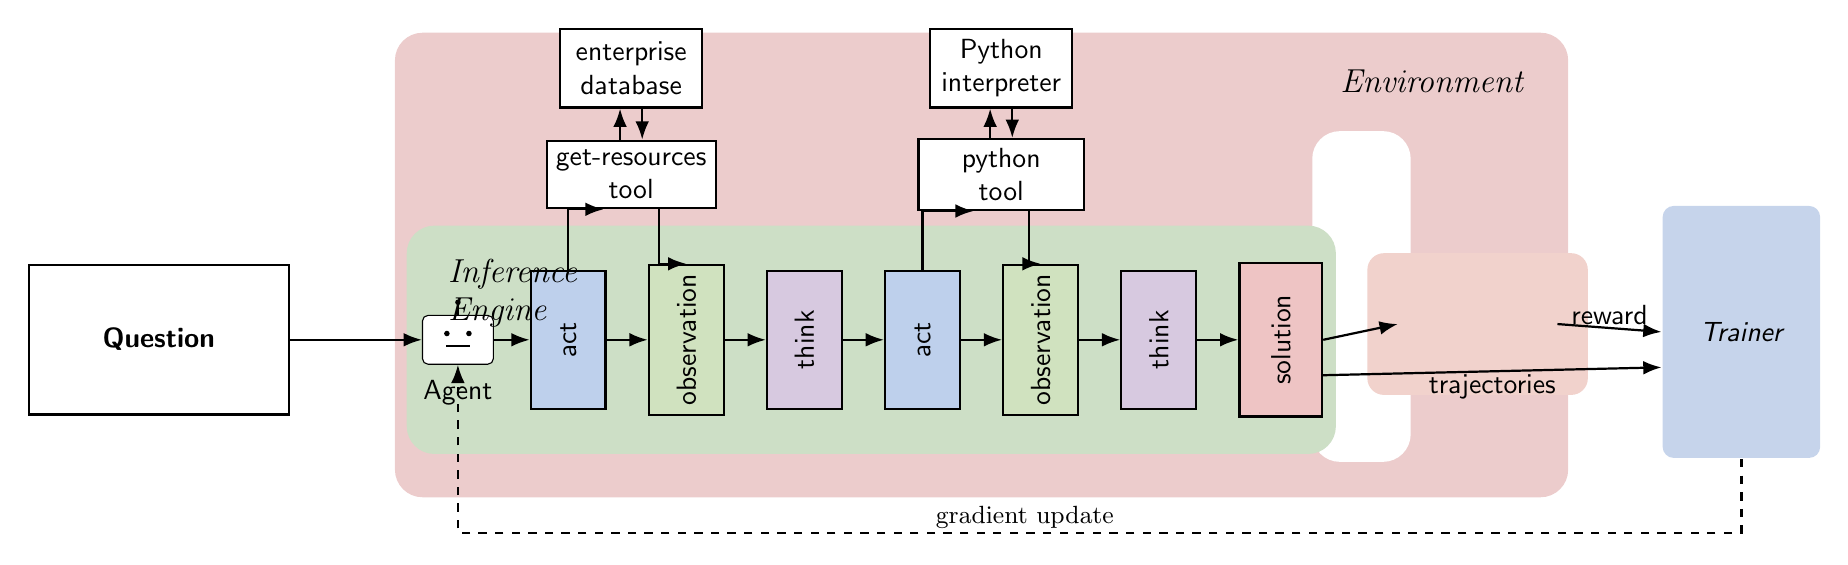
\begin{tikzpicture}[>=Latex, font=\sffamily]
  \tikzset{
    flow/.style={-Latex, thick},
    proc/.style={draw, thick, minimum width=0.95cm, minimum height=1.75cm, align=center},
    tool/.style={draw, thick, fill=white, minimum width=2.1cm, minimum height=0.85cm, align=center},
    smallbox/.style={draw, thick, rounded corners=4pt, fill=white, minimum width=1.8cm, minimum height=1.0cm, align=center}
  }

  % Main nodes
  \node[draw, thick, fill=white, minimum width=3.3cm, minimum height=1.9cm, align=center] (question) at (0,0) {\textbf{Question}};

  \node[draw, rounded corners=2pt, fill=white, minimum width=0.9cm, minimum height=0.62cm] (agent) at (3.8,0) {};
  \draw[thick] (agent.north) -- ++(0,0.13);
  \fill ($(agent.north)+(0,0.16)$) circle (1pt);
  \fill ($(agent.center)+(-0.14,0.08)$) circle (1pt);
  \fill ($(agent.center)+(0.14,0.08)$) circle (1pt);
  \draw[thick] ($(agent.center)+(-0.15,-0.08)$) -- ($(agent.center)+(0.15,-0.08)$);
  \node[below=2pt of agent] (agentlbl) {Agent};

  \node[proc, fill=actblue]        (act1)   at (5.2,0) {\rotatebox{90}{act}};
  \node[proc, fill=obsgreen]       (obs1)   at (6.7,0) {\rotatebox{90}{observation}};
  \node[proc, fill=thinkviolet]    (think1) at (8.2,0) {\rotatebox{90}{think}};
  \node[proc, fill=actblue]        (act2)   at (9.7,0) {\rotatebox{90}{act}};
  \node[proc, fill=obsgreen]       (obs2)   at (11.2,0) {\rotatebox{90}{observation}};
  \node[proc, fill=thinkviolet]    (think2) at (12.7,0) {\rotatebox{90}{think}};
  \node[proc, fill=solred, minimum width=1.05cm, minimum height=1.95cm] (solution) at (14.25,0) {\rotatebox{90}{solution}};

  \node[tool] (getres) at (6.0,2.1) {get-resources\\tool};
  \node[tool] (pyt)    at (10.7,2.1) {python\\tool};
  \node[tool, minimum width=1.8cm, minimum height=1.0cm] (edb) at (6.0,3.45) {enterprise\\database};
  \node[tool, minimum width=1.8cm, minimum height=1.0cm] (pyi) at (10.7,3.45) {Python\\interpreter};

  \node[smallbox, fill=judgepink, minimum width=2.0cm, minimum height=1.1cm] (judge) at (16.75,0.2) {Judge};
  \node[draw=none, fill=judgepink, rounded corners=6pt, minimum width=2.8cm, minimum height=1.8cm] (judgebg) at (16.75,0.2) {};
  \node[smallbox, fill=trainerblue, draw=none, minimum width=2.0cm, minimum height=3.2cm] (trainer) at (20.1,0.1) {\itshape Trainer};

  % Background regions
  \begin{scope}[on background layer]
    \fill[rounded corners=10pt, fill=envpink] (3.0,-2.0) rectangle (17.9,3.9);
    \fill[rounded corners=10pt, fill=white] (14.65,-1.55) rectangle (15.9,2.65);
    \fill[rounded corners=10pt, fill=infgreen] (3.15,-1.45) rectangle (14.95,1.45);
  \end{scope}

  % Labels inside regions
  \node[anchor=north west, font=\itshape\large, align=left] at (3.55,1.15) {Inference\\Engine};
  \node[anchor=north east, font=\itshape\large] at (17.45,3.55) {Environment};

  % Flow arrows
  \draw[flow] (question.east) -- (agent.west);
  \draw[flow] (agent.east) -- (act1.west);
  \draw[flow] (act1.east) -- (obs1.west);
  \draw[flow] (obs1.east) -- (think1.west);
  \draw[flow] (think1.east) -- (act2.west);
  \draw[flow] (act2.east) -- (obs2.west);
  \draw[flow] (obs2.east) -- (think2.west);
  \draw[flow] (think2.east) -- (solution.west);

  \draw[flow] (solution.east) -- (judge.west);
  \draw[flow] (judge.east) -- node[above, inner sep=1pt] {reward} (trainer.west);
  \draw[flow] ([yshift=-0.45cm]solution.east) -- node[below, inner sep=1pt] {trajectories} ([yshift=-0.45cm]trainer.west);

  % Tool connections
  \draw[flow] ([xshift=-4pt]getres.north) -- ([xshift=-4pt]edb.south);
  \draw[flow] ([xshift=4pt]edb.south) -- ([xshift=4pt]getres.north);
  \draw[flow] ([xshift=-4pt]pyt.north) -- ([xshift=-4pt]pyi.south);
  \draw[flow] ([xshift=4pt]pyi.south) -- ([xshift=4pt]pyt.north);

  \draw[flow] (act1.north) |- ([xshift=-0.35cm]getres.south);
  \draw[flow] ([xshift=0.35cm]getres.south) |- (obs1.north);
  \draw[flow] (act2.north) |- ([xshift=-0.35cm]pyt.south);
  \draw[flow] ([xshift=0.35cm]pyt.south) |- (obs2.north);

  % Gradient update loop
  \draw[dashed, flow] (trainer.south) |- (8.9,-2.45) -| (agent.south);
  \node[font=\small] at (11.0,-2.25) {gradient update};

\end{tikzpicture}
\end{document}